%%%%%%%%%%%%%%%%%%%%%%%%%%%%%%%%%%%%%%%%%
% Beamer Presentation
% LaTeX Template
% Version 1.0 (10/11/12)
%
% This template has been downloaded from:
% http://www.LaTeXTemplates.com
%
% License:
% CC BY-NC-SA 3.0 (http://creativecommons.org/licenses/by-nc-sa/3.0/)
%
%%%%%%%%%%%%%%%%%%%%%%%%%%%%%%%%%%%%%%%%%

%----------------------------------------------------------------------------------------
%	PACKAGES AND THEMES
%----------------------------------------------------------------------------------------

\documentclass{beamer}

\mode<presentation> {

% The Beamer class comes with a number of default slide themes
% which change the colors and layouts of slides. Below this is a list
% of all the themes, uncomment each in turn to see what they look like.

%\usetheme{default}
%\usetheme{AnnArbor}
%\usetheme{Antibes}
%\usetheme{Bergen}
%\usetheme{Berkeley}
%\usetheme{Berlin}
%\usetheme{Boadilla}
%\usetheme{CambridgeUS}
%\usetheme{Copenhagen}
%\usetheme{Darmstadt}
%\usetheme{Dresden}
%\usetheme{Frankfurt}
%\usetheme{Goettingen}
%\usetheme{Hannover}
\usetheme{Ilmenau}
%\usetheme{JuanLesPins}
%\usetheme{Luebeck}
%\usetheme{Madrid}
%\usetheme{Malmoe}
%\usetheme{Marburg}
%\usetheme{Montpellier}
%\usetheme{PaloAlto}
%\usetheme{Pittsburgh}
%\usetheme{Rochester}
%\usetheme{Singapore}
%\usetheme{Szeged}
%\usetheme{Warsaw}

% As well as themes, the Beamer class has a number of color themes
% for any slide theme. Uncomment each of these in turn to see how it
% changes the colors of your current slide theme.

%\usecolortheme{albatross}
%\usecolortheme{beaver}
%\usecolortheme{beetle}
%\usecolortheme{crane}
%\usecolortheme{dolphin}
%\usecolortheme{dove}
%\usecolortheme{fly}
%\usecolortheme{lily}
%\usecolortheme{orchid}
%\usecolortheme{rose}
%\usecolortheme{seagull}
%\usecolortheme{seahorse}
%\usecolortheme{whale}
%\usecolortheme{wolverine}

%\setbeamertemplate{footline} % To remove the footer line in all slides uncomment this line
%\setbeamertemplate{footline}[page number] % To replace the footer line in all slides with a simple slide count uncomment this line

\setbeamertemplate{navigation symbols}{} % To remove the navigation symbols from the bottom of all slides uncomment this line
}


\usepackage{graphicx} % Allows including images
\usepackage{booktabs} % Allows the use of \toprule, \midrule and \bottomrule in tables
%\usepackage{bibentry}
%\usepackage{natbib}
\usepackage[T2A]{fontenc} % enable Cyrillic fonts
\usepackage[utf8]{inputenc} % make weird characters work
\usepackage{epigraph}
\usepackage[english,serbian]{babel}

%----------------------------------------------------------------------------------------
%	TITLE PAGE
%----------------------------------------------------------------------------------------

\title[Pouzdanost Softvera]{Implementirano $\neq$ testirano $\neq$ ispravno} % The short title appears at the bottom of every slide, the full title is only on the title page

\author{Nenad Ajvaz, Stefan Kapunac,\\ Filip Jovanović, Aleksandra Radosavljević} % Your name
\institute[MATF] % Your institution as it will appear on the bottom of every slide, may be shorthand to save space
{
Univerzitet u Beogradu, Matematički Fakultet \\ % Your institution for the title page
\medskip
}
\date{19.5.2019.} % Date, can be changed to a custom date

\begin{document}

\begin{frame}
\titlepage % Print the title page as the first slide
\end{frame}

\begin{frame}
\frametitle{Pregled} % Table of contents slide, comment this block out to remove it
\tableofcontents % Throughout your presentation, if you choose to use \section{} and \subsection{} commands, these will automatically be printed on this slide as an overview of your presentation
\end{frame}

%----------------------------------------------------------------------------------------
%	PRESENTATION SLIDES
%----------------------------------------------------------------------------------------


\section{Uvod}
\begin{frame} 
\frametitle{Primena softvera u svakodnevnom životu}
\textbf{Softver se danas koristi doslovno svuda}

\begin{columns}[c] % The "c" option specifies centered vertical alignment while the "t" option is used for top vertical alignment
\column{.45\textwidth}
\begin{itemize}
\item Administracija
\item Edukacija
\item Komunikacija
\item Industrija
\item Saobraćaj
\end{itemize}

\column{.45\textwidth}
\begin{itemize}
\item Ekonomija
\item Zdravstvo
\item Nauka
\item Inženjerstvo
\item ...
\end{itemize}
\end{columns}
\end{frame}

\begin{frame}
\frametitle{Primeri neispravnog softvera}

\begin{columns}[c] % The "c" option specifies centered vertical alignment while the "t" option is used for top vertical alignment

\column{.45\textwidth}
\begin{itemize}
\item Therac-25, 1985.
\item Marsov orbiter za proučavanje klime, 1999.
\item Letovi u Los Anđelesu, 2004.
\item Boing 737 MAX, 2019.
\end{itemize}

\column{.3\textwidth}

\begin{figure}
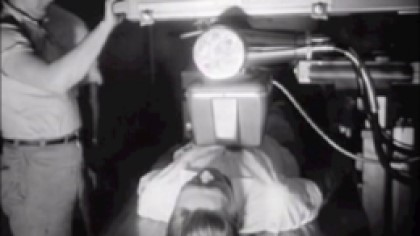
\includegraphics[width=1\linewidth]{therac.jpg}
\end{figure}

\begin{figure}
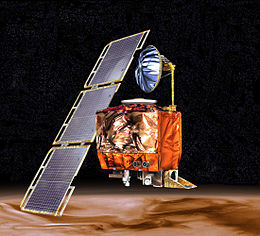
\includegraphics[width=1\linewidth]{MCO.jpg}
\end{figure}

\end{columns}
\end{frame}

\section{Verifikacija}
\begin{frame}
\frametitle{Testiranje u razvoju softvera}
\begin{columns}[c] % The "c" option specifies centered vertical alignment while the "t" option is used for top vertical alignment
\column{.45\textwidth}
\begin{figure}
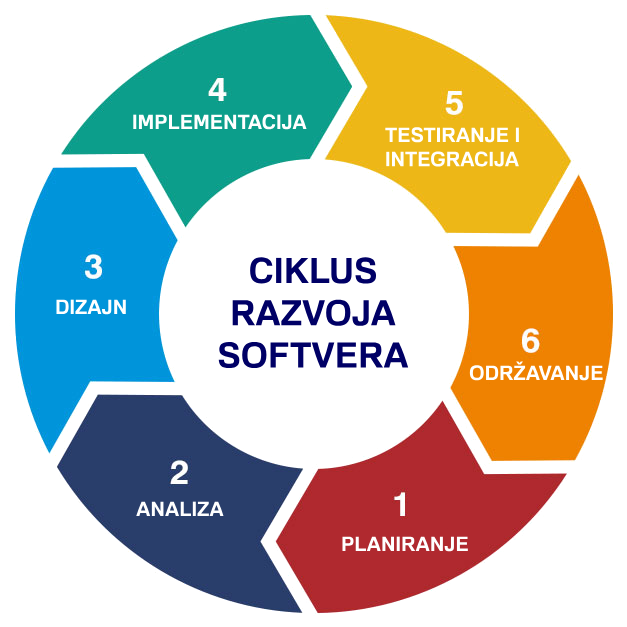
\includegraphics[width=1\linewidth]{rs.png}
\end{figure}

\column{.45\textwidth}
\epigraph{\emph{,,Program testing can be used to show the presence of bugs, but never to show their absence!‘‘}}{Edsger W. Dijkstra}

\end{columns}
\end{frame}


\begin{frame}
\frametitle{Verifikacija softvera}

\textbf{Definicija}
\begin{itemize}
\item \textit{verification = Are we building the product right?}
\item \textit{validation = Are we building the right product?}
\end{itemize}

\textbf{Podela}
\begin{enumerate}
\item Dinamička verifikacija
\begin{itemize}
\item testiranje crne kutije (funkcionalno testiranje)
\item testiranje bele kutije (strukturno testiranje)
\end{itemize}
\item Statička verifikacija
\begin{itemize}
\item simboličko izvršavanje
\item aptraktna interpretacija
\end{itemize}
\end{enumerate}
\end{frame}


\begin{frame}
\frametitle{Alati za verifikaciju softvera}

\begin{itemize}
\item \textbf{Alati za automatsko testiranje} \\
\textit{Obezbeđuju automatsko sprovođenje testova}
\begin{itemize}
\item Selenium
\item ...
\end{itemize}
\item \textbf{Formalni dokazivači ispravnosti} \\
\textit{Omogućavaju interaktivnu formulaciju matematičkog dokaza korektnosti}
\begin{itemize}
\item Isabelle/HOL
\item Coq
\item ...
\end{itemize}
\end{itemize}
\end{frame}

\section{Modeli i metrike}
\begin{frame}
\frametitle{Modeli i metrike pouzdanosti}

\begin{enumerate}
\item Deterministički modeli
\begin{itemize}
\item Holstedova metrika
\item Mek-Kejbova ciklomatična složenost
\item ...
\end{itemize}
\item Probabilistički modeli
\begin{itemize}
\item Modeli stope neuspeha
\item Modeli rasta pouzdanosti
\item ...
\end{itemize}
\end{enumerate}

\end{frame}


\begin{frame}
\frametitle{Holstedova metrika}

\begin{itemize}
\item Meri se kompleksnost programa
\item Broj operatora i operanada se dovodi u vezu sa pojavom bagova
\end{itemize}

\end{frame}


\begin{frame}
\frametitle{Mek-Kejbova ciklomatična složenost}

\begin{columns}[c] % The "c" option specifies centered vertical alignment while the "t" option is used for top vertical alignment


\column{.45\textwidth}

\begin{center}
\textbf{C = E - V + 2P} 
\end{center}

E = broj grana grafa G \\
V = broj čvorova grafa G \\
P = broj povezanih komponenti grafa G \\
G = graf kontrole toka programa 

\column{.45\textwidth}
\begin{figure}
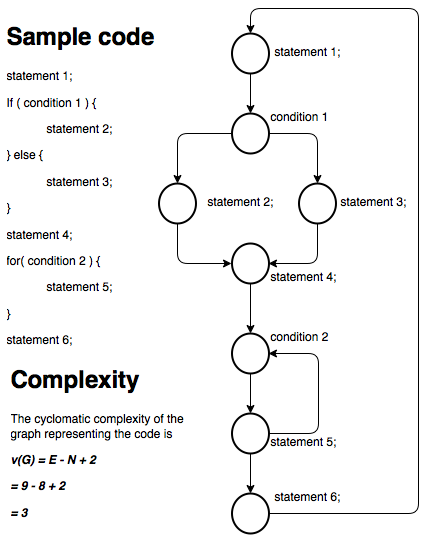
\includegraphics[width=1\linewidth]{mccabe.png}
\end{figure}

\end{columns}

\end{frame}


\begin{frame}
\frametitle{Probabilistički modeli}

\begin{itemize}

\item Greška kao verovatnosni događaj
\item Razne metode iz oblasti statistike

\end{itemize}

\textbf{Podela}
\begin{enumerate}
\item Moteli stope neuspeha
\begin{itemize}
\item prikazuju stopu otkazivanja programa po pojavi greške
\item nekoliko varijacija ovih modela
\item ...
\end{itemize}
\item Modeli rasta pouzdanosti
\begin{itemize}
\item predviđaju da li dolazi do poboljšanja pouzdanosti kroz testiranje softvera
\item dva podmodela
\item ...
\end{itemize}
\end{enumerate}

\end{frame}

\section{Budućnost}
\begin{frame}
\frametitle{Budućnost softvera}

Razni alati već danas automatizuju mnoge faze razvoja
\begin{itemize}
\item Generisanje koda
\item Optimizacija
\item Debagovanje
\end{itemize}
\end{frame}

\begin{frame}
\frametitle{Veštačka inteligencija}

\begin{itemize}
\item Sa napretkom veštačke inteligencije i mašinskog učenja, proces razvoja može da se ubrza eksponencijalno
\item Već se radi na sistemima koji automatski generišu kod (Bayou)
\item Verujemo da će u budućnosti kod da pišu mašine, a zadatak programera će biti samo da ih kontroliše i usmerava
\end{itemize}
\end{frame}

\section{Zaključak}
\begin{frame}
\frametitle{Zaključak}
\begin{enumerate}
\item Greške su neizbežne
\item Testiranje je važno, ali ne uvek i dovoljno
\item Formalna verifikacija je ponekad neophodna
\item Mašine će zavladati svetom
\end{enumerate}
\end{frame}

\section{Literatura}
\begin{frame}

\nocite{quinn_ethics}
\nocite{laski2009software}
\nocite{pham_reliability}
\nocite{Bayou}

\frametitle{Literatura}
\bibliographystyle{ieeetr}
\bibliography{seminarski}
\end{frame}

\end{document} 